% !TEX root = ../thesis.tex
\chapter{Konfigurácia prostredia, metodika testovania a merania}
\section{Prostredie virtuálnych strojov pomocou VirtualBox}\label{merania}
Pri testovaní funkcionality VPN sme použili virtualizačný nástroj (daľej \acrshort{vm}) Virtual Box (ďalej \acrshort{vb}), spoločnosti Oracle, vo verzii 6.1.30. \acrshort{vb} je voľne dostupný. Inštalácia je jednoduchá a rýchla. Viac informácii o nástroji je možné dohľadať v \cite{vbox}.

Pre použitie je potrebné aby mal používateľ k dispozícií obraz operačného systému (ďalej \acrshort{os}). Tie nie je problém získať ani pre \acrshort{os} Windows a podobne, avšak pri našej práci sme zvolili využitie voľno dostupného  \acrshort{os} -- \textbf{Linux Ubuntu} vo verziách 20.04.3(\acrshort{lts}\footnote{z ang. \acrlong{lts}})-- OSC a 21.10 -- OSS. Pri opise práce použijeme označenia OSS pre VPN server a OSC pre klienta.

Pri jednoduchej inštalácií \acrshort{vm} sme použili konfiguráciu s  2048 MB RAM a 2 jadrami. (Minimálna inštalácia). V prípade potreby dávame do popredia návod na prípravu Windows \acrshort{os} v \acrshort{vm} -- \cite{vmkonfig}, avšak postup je triviálny. Po inštalácii sme OS aktualizovali pomocou príkazov:
\begin{lstlisting}[language=bash]
	sudo apt-get update
	sudo apt-get upgrade
\end{lstlisting}
Následne sme doinštalovali potrebné súčasti k \acrshort{vm} \acrshort{os} vo verzii ako je \acrshort{vb}, teda 6.1.30. Dôvodom bolo zväčšenie rozlíšenia a využívanie možnosti zdieľaného priečinka s \acrshort{os}, na ktorom daný \acrshort{vb} beží. Za účelom správneho fungovania priečinka bolo nutné v termináli použiť príkaz:
\begin{lstlisting}[language=bash]
	sudo usermod -aG vboxsf $(whoami)
\end{lstlisting}
a následne reštartovať \acrshort{os}.

Posledné úpravy prostredia sú spojené s jazykom C a balíčkom Make. Inštalácia je opäť jednoduchá. Použili sme príkazy:
\begin{lstlisting}[language=bash]
	sudo apt install gcc
	sudo apt install make
\end{lstlisting}
Uvedené úpravy boli vykonané na oboch \acrshort{os}.

V prípade použitia \acrshort{os} Windows je postup inštalácie jazyka C a balička Make zložitejší. Používateľovi odporúčam použitie knižníc Winlibs, dostupne na \href{https://winlibs.com/}{webe}. Po stiahnutí balíčkov musí používateľ importovať uvedený balíček, resp. cestu k nemu, do premenných prostredia \acrshort{os} Windows. Jeden zo spôsobov je uvedený aj na Winlibs stránke. 

\section{Zmena sieťových adaptérov}
\acrshort{vb} ponúka rôzne možnosti nastavenia sieťových adaptérov. Aktuálne su dostupné tieto:
\begin{itemize}
	\item{Not attached}
	\item{Network Address Translation (ďalej NAT)}
	\item{NAT Network}
	\item{Bridge adapter}
	\item{Internal}
	\item{Host-Only}
	\item{Generic driver}
	\item{Cloud-Based} -- experimentálne
\end{itemize} 
 
Konektivita jednotlivých možností je znázornená pomocou obrázku \ref{vbmode}. Viac informácií o jednotlivých režimoch je dostupných na \cite{vboracle}.

\begin{figure}
	\centering
	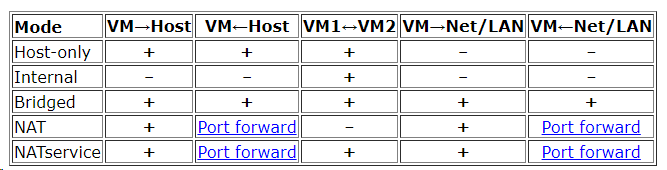
\includegraphics[width=.9\textwidth]{figures/vbmodes}
	\caption{Konektivita jednotlivých sieťových adaptérov}
	\label{vbmode}
\end{figure}
Vzhľadom k našim potrebám, teda obojsmerná komunikácia medzi 2 VM, sú pre nás relevantné režimy bridge a NAT network. Ako si môžeme všimnúť, NAT vyžaduje dodatočnú konfiguráciu portov v prípadoch kedy chceme aby nastala komunikácia medzi dvoma VM. Z tohto dôvodu je pre čo najjednoduchší prístup zvoliť práve režim bridge. Ten priradí VM vlastnú IP adresu, pomocou, ktorej stroj komunikuje. 

Viac o jednotlivých režimov je taktiež možné nájsť v \cite{vbguide}. Autor sa venuje postupu konfigurácie jednotlivých režimov spoločne s ich opisom.

\section{Nástroje použité v obrazoch}
  winlibs, visual studio , gcc ,make, c kod na meranie poctu cyklov z bc + cas  
\chapter{Implementacia jednoduchej VPN siete}
https://learn.microsoft.com/en-us/windows/win32/winsock/finished-server-and-client-code
\section{Dead Simple VPN}\label{dsvpn}
Dead Simple VPN je voľne dostupný\footnote{\href{https://github.com/jedisct1/dsvpn}{https://github.com/jedisct1/dsvpn}} program, napísaný v jazyku C. Určený je pre operačný systém Linux. Autorom je Frank Denis. DSVPN rieši najbežnejší prípad použitia VPN, teda pripojenie klienta k VPN serveru cez nezabezpečenú sieť. Následne sa klient dostane na internet prostredníctvom servera. Uvedenú skutočnosť je možne vidieť na schéme \ref{vpnsimple}.
\begin{figure}
	\centering
	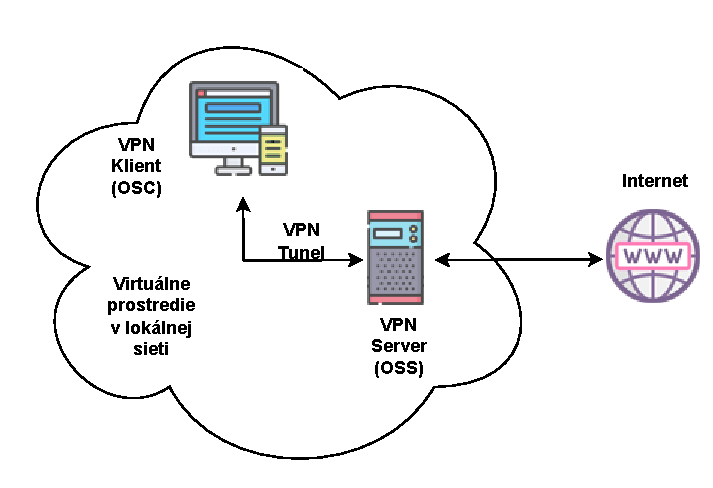
\includegraphics[width=0.9\textwidth]{figures/vpnsimple}
	\caption{Schéma jednoduchej VPN}
	\label{vpnsimple}
\end{figure}


DSVPN používa protokol riadenia prenosu -- \acrshort{tcp}\footnote{z ang. \textit{Transmission Control Protocol}} \cite{tcp}. Medzi ďalšie pozitíva patrí:
\begin{itemize}
	\item{Používa iba modernú kryptografiu s formálne overenými implementáciami,}
	\item{Malá a konštantná pamäťová stopa. Nevykonáva žiadne dynamické alokovanie pamäte (z ang. \textit{heap memory}),}
	\item{Malý (~25 KB) a čitateľný kód. Žiadne vonkajšie závislosti (z ang. \textit{Dependencies}),}
	\item{Funguje po preklade GCC prekladačom. Bez dlhej dokumentácia, žiaden konfiguračný súbor, dodatočná konfigurácia. DSVPN je spustiteľná jednoriadkovým príkazom na serveri, obdobne na klientovi. Bez potreby konfigurácie brány firewall a pravidiel smerovania,}
	\item{Funguje na Linuxe (kernel >= 3.17), macOS a OpenBSD, DragonFly BSD, FreeBSD a NetBSD v klientskych a point-to-point režimoch. Pridanie podpory pre iné operačné systémy je triviálne,}
	\item{Nedochádza k úniku IP medzi pripojeniami, ak sa sieť nezmení. Blokuje IPv6 na klientovi, aby sa zabránilo úniku IPv6 adries.}
\end{itemize} 

V uvedenej VPN autor zakomponoval aj možnosť pokročilejších nastavení. Celkový súhrn vstupných parametrov pri štarte programu je takýto:
\begin{lstlisting}[language=bash]
	./dsvpn   server
	<key file>
	<vpn server ip or name>|"auto"
	<vpn server port>|"auto"
	<tun interface>|"auto"
	<local tunnel ip>|"auto"
	<remote tunnel ip>"auto"
	<external ip>|"auto"

	./dsvpn   client
	<key file>
	<vpn server ip or name>
	<vpn server port>|"auto"
	<tun interface>|"auto"
	<local tunnel ip>|"auto"
	<remote tunnel ip>|"auto"
	<gateway ip>|"auto"
	\end{lstlisting} 
Väčšina parametrov je však prednastavených na automatické hodnoty. Príkladom je port 443, vytvorenie rozhrania tun0, prevziatie externej IP adresy zo siete a ďalšie. 

\section{Kryptografia použitá v DSVPN}
DSVPN používa v svojej implementácií malú sebestačnú kryptografickú knižnicu -- \textit{Charm}\footnote{\url{https://github.com/jedisct1/charm}}. Jej autorom je tvorca DSVPN. Implementácia umožňuje autentizované šifrovanie (z ang.\textit{authenticated encryption}) a hašovanie kľúčov (z ang. \textit{keyed hashing}). Správnosť implementácie algoritmu v knižnici programátor overil pomocou nástroja \textbf{Cryptol}\footnote{\url{https://cryptol.net/index.html}}. Uvedený nástroj slúži na zápis algoritmu do matematickej špecifikácií. Tým poskytne možnosť jednoduchšej a hlavne korektnej implementácie zvoleného kryptografického algoritmu. Zároveň je možné program využiť aj na verifikáciu vytvoreného riešenia. Obdobne sú v repozitári knižnice ponechané overovacie skripty pre jednoduché spustenie. 

Kryptografický algoritmus použitý v DSVPN je Xoodoo permutácia v duplex móde, pričom môže byť jednoducho nahradená napríklad Gimli-im\footnote{\url{https://github.com/jedisct1/gimli}} \cite{gimli} alebo Simpira384\footnote{\url{https://github.com/jedisct1/simpira384}} \cite{simpira}, ktorá je založené na AES-e . Uvedené algoritmy sú predmetom opisu kapitoly \ref{krypto}. Pri zmene musí používateľ zasiahnuť do zdrojového kódu v súbore \textbf{charm.c}, ktorého obsahom sú kryptografické primitíva.     
\section{Experimentálne overenie VPN}
DSVPN sme prakticky overili pomocou dvojice virtuálnych strojov OSS a OSC, ktorých opis je obsahom \ref{merania}. Na zariadení OSS sme pomocou balička make a GCC prekladača vykonali inštaláciu DSVPN. Obdobný postup je aplikovaný aj vo VM OSC. Na OSS spúšťame VPN Server, ktorý nám poskytne IP adresu, prostredníctvom ktorej budeme komunikovať s vonkajším svetom. Na spustenie a vytvorenie spojenie vykonáme nasledujúce úkony:
\begin{enumerate}
	\item Vygenerovanie zdieľaného kľúča:\begin{lstlisting}[language=bash]
		dd if=/dev/urandom of=vpn.key count=1 bs=32
	\end{lstlisting} 
-- zdieľaný kľúč, ktorý sme vygenerovali, sa nám uložil do súboru \textit{vpn.key}. Ten je potrebné vložiť do priečinka s programom \textit{dsvpn} v oboch zariadeniach -- OSS aj OSC. 
	\item OSS zariadenie: \begin{lstlisting}[language=bash] 
	sudo ./dsvpn server vpn.key auto 
	2340 auto 10.8.0.254 10.8.0.2
	\end{lstlisting} 
-- tento príkaz zabezpečí spustenie VPN servera na prostredí OSS s IP adresou, priradenou k vytvoren=emu tunelovaciemu rozhraniu s menom \textit{tun0}. Vytvorí sa pri spustení servera\footnote{Pomocou \lstinline|ip address show tun0| zistíme IPv4 adresu VPN servera.}. Príkazom ďalej definujeme portové číslo 2340, ktoré sa použije pri nastolení TCP spojenie medzi klientom a serverom. Poslednou konfiguráciou je priradenie IP adresy tunelov, ktoré bude využívať náš klient -- 10.8.0.254 a server -- 10.8.0.2. Používateľ má ešte možnosť nastaviť tzv. External IP. Tú by sme využili ak by sme spúšťali DSVPN na routri poskytovateľa internetu.  
	\item OSC zariadenie: \begin{lstlisting}[language=bash] 
	sudo ./dsvpn client vpn.key 192.168.88.62 
	2340 auto 10.8.0.2 10.8.0.254
	\end{lstlisting} 
-- uvedený príkaz zabezpečí, že sa pripojíme na VPN Server, ktorý ma ip adresu \textit{192.168.88.62} s portom 2340. Následne vzniká TCP spojenie. Dôležité je si všimnúť poradie adries tunelov. Je opačné ako v prípade servera. 
	\item V prípade úspešnej konektivity sa operácia podarila a pre okolitý svet sme viditelný pomocou IP adresy, ktorú sme zvolili. 
\end{enumerate}

Na overenie správnosti funkcionality nám postačí jednoduchý sieťový príkaz \lstinline|traceroute|. Napríklad \lstinline|traceroute google.sk|\footnote{vo Windows CMD prostredí: \lstinline|tracert google.sk|}. Prvá z uvedených adries je práve tá, ktorú dané zariadenie používa. 

V našom prípade bolo nutné použiť lokálne adresy vzhľadom na to, že obe VM bežia na jednom hosťovskom počítači. Obidva zariadenia sú tým pádom pripojené k jednému internetovému poskytovateľovi, čo má za následok takmer rovnaké smerovanie k vzdialenej doméne. 

Proces zistenia IP adresy VPN servera, po spustení, a overenie funkčnosti je následne znázornené pomocou \ref{ipu21},\ref{ipu20}, \ref{vpntru20}.
V  \ref{ipu21} sme žltou farbou znázornili IP adresu, na ktorej je VPN server dostupný. Oranžová farba znázorňuje IP adresy tunelu medzi serverom a klientom v tomto poradí. Následne v \ref{ipu20} môžeme vidieť to isté pre klienta.
  \begin{figure}
  	\centering
  	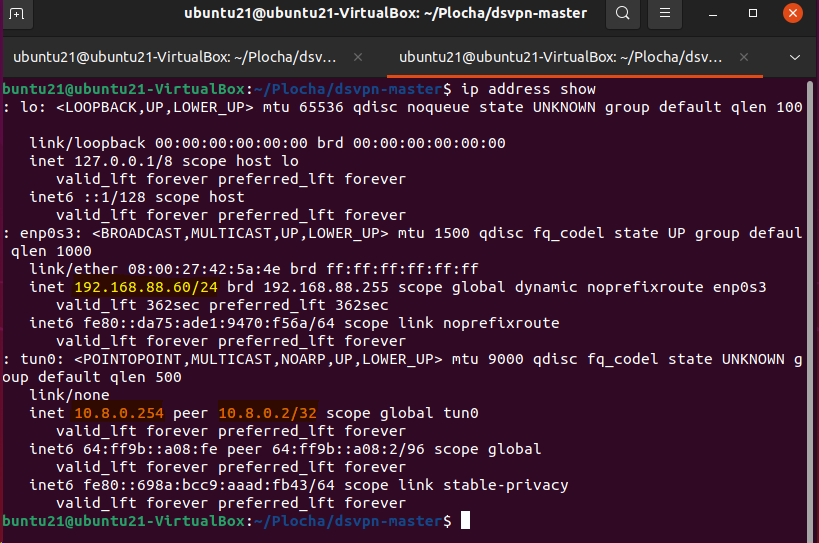
\includegraphics[width=0.9\textwidth]{figures/ipu21}
  	\caption{Zistenie IP adries VPN Servera na VM OSS}
  	\label{ipu21}
  \end{figure}
  

\begin{figure}
	\centering
	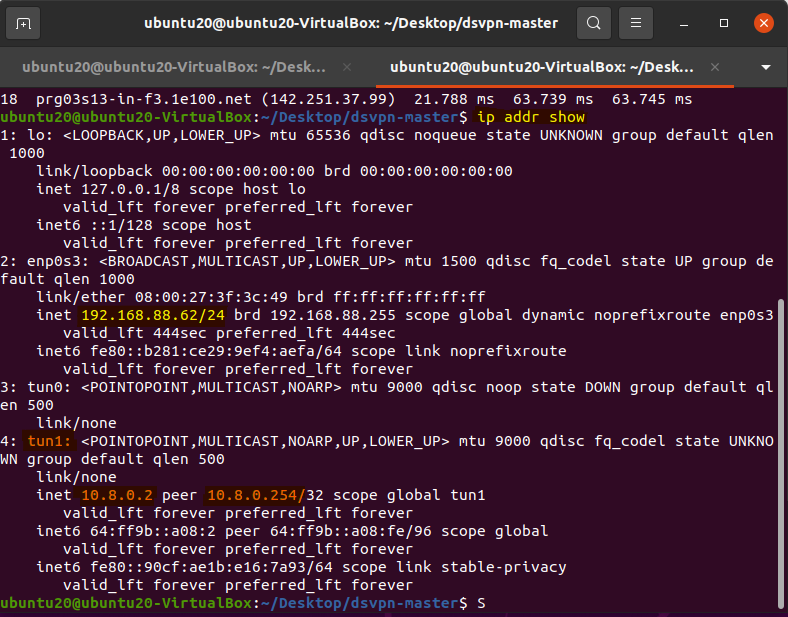
\includegraphics[width=0.9\textwidth]{figures/ipu20}
	\caption{Zistenie IP adries VPN Klienta na VM OSC}
	\label{ipu20}
\end{figure}
Nakoniec, v \ref{vpntru20} môžeme vidieť ako klient pri internetovej komunikácií používa namiesto svojej vlastnej, adresu poskytnutú VPN Serverom na zariadení OSS -- žltou zvýraznená IP. Červenou je zaškrnutá farba poskytovateľa internetu. 

\begin{figure}
	\centering
	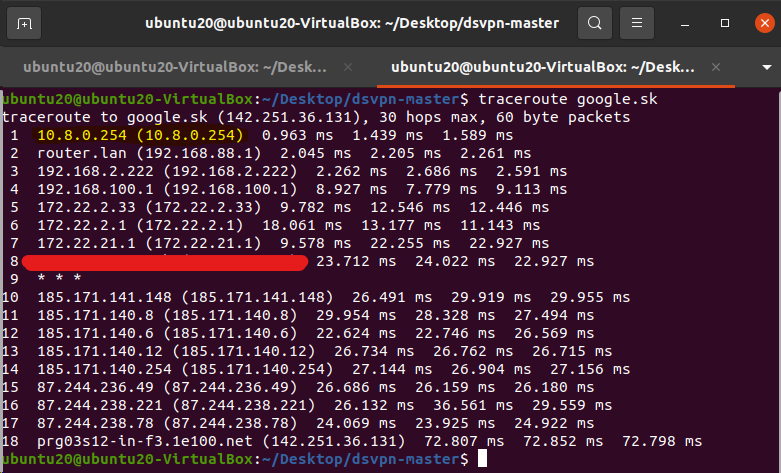
\includegraphics[width=0.9\textwidth]{figures/vpntru20}
	\caption{Overenie funkcionality DSVPN pomocou traceroute}
	\label{vpntru20}
\end{figure}
\section{Princíp fungovania programu}
High level overview

\section{Analýza zdrojového kódu DSVPN}
 Pri analýze sa zameriame výhradne na dôležité časti kódu DSVPN pre programovací jazyk C. Repozitár pozostáva z jedného make-file balíčka\cite{make}. 3 hlavičkových (.h) a k ním korešpondujúcimi zdrojovými kódmi (.c), s pomenovaním:
 \begin{enumerate}
 	\item \textbf{charm.h} -- kryptografická knižnica so 6 funkciami,
 	\item \textbf{os.h} -- funkcie čítania a zápisu paketov, vytvorenia, aplikácie a zrušenia tunelu,
 	\item \textbf{vpn.h} -- deklarácia konštánt, endianity\cite{endianita} a niektorých závislostí OS.
 \end{enumerate}

 V spomenutých hlavičkových súboroch sa nachádzajú deklarácie funkcií, ktoré VPN používa. Definície sú obsahom .c súborov, ako je v jazyku C zaužívaným zvykom. Obsahom tejto podkapitoly je analýza týchto kódov. 
 
 \subsection{Súbor charm.h a charm.c}
 Obsahom sú prevažne funkcie slúžiace pri behu kryptografického algoritmu XOODOO. Charm.h pozostáva z 6 funkcií. Ich implementácia nie je až tak rozsiahla. Zaberá celkovo 337 riadkov. Jednotlivú implementáciu každej funkcie postupne opíšeme. 
 
   \begin{minipage}{\linewidth} 	
  	\begin{lstlisting}[frame=single,
  		numbers=left,
  		caption={Obsah charm.h}\label{charm.h},
  		basicstyle=\ttfamily\small, keywordstyle=\color{black}\bfseries,]
void uc_state_init(uint32_t st[12], const unsigned char key[32], 
				  			 	 const unsigned char iv[16]);
void uc_encrypt(uint32_t st[12], unsigned char *msg, 
							  size_t msg_len, unsigned char tag[16]);	
int uc_decrypt(uint32_t st[12], unsigned char *msg, 
			   			   size_t msg_len,
			   			   const unsigned char *expected_tag, 
			   			   size_t expected_tag_len);
void uc_hash(uint32_t st[12], unsigned char h[32],
			 			 const unsigned char *msg, size_t len);
void uc_memzero(void *buf, size_t len);
void uc_randombytes_buf(void *buf, size_t len);
  		 	\end{lstlisting}
  	\end{minipage}\\
 \subsection{Súbor os.h a os.c}
 Obsahom su funkcie, ktorých úlohami sú čítanie alebo pridanie \acrshort{gw}, vytvorenie a nastavenie tunelu v danom OS. Následne je aplikovaná úprava firewall pravidiel, tak aby všetka komunikácia bola presmerovaná na VPN server. Úprava firewall pravidiel je závislá od role, pod ktorou je VPN spustená. Teda či sa jedná o server alebo klienta. 
 Celkovo je obsahom 12 funkcií, ktoré riešia uvedené úlohy. Detail je možné vidiet v \ref{os.h}.
 
 \begin{minipage}{\linewidth} 	
	\begin{lstlisting}[frame=single,
		numbers=left,
		caption={Obsah ZK os.h}\label{os.h},
		basicstyle=\ttfamily\small, keywordstyle=\color{black}\bfseries,]
 ssize_t safe_read(const int fd, void *const buf_, size_t count, 
 						       const int timeout);
 ssize_t safe_write(const int fd, const void *const buf_, 
 							      size_t count,
 							      const int timeout);
 ssize_t safe_read_partial(const int fd, void *const buf_,
 							 					   const size_t max_count);
 ssize_t safe_write_partial(const int fd, void *const buf_, 
 							    		     	const size_t max_count);
 
 typedef struct Cmds {
 	const char *const *set;
 	const char *const *unset;
 } Cmds;
 
 Cmds firewall_rules_cmds(int is_server);
 int shell_cmd(const char *substs[][2], const char *args_str,
 			         int silent);
 const char *get_default_gw_ip(void);
 const char *get_default_ext_if_name(void);
 int tcp_opts(int fd);
 int tun_create(char if_name[IFNAMSIZ], const char *wanted_name);
 int tun_set_mtu(const char *if_name, int mtu);
 ssize_t tun_read(int fd, void *data, size_t size);
 ssize_t tun_write(int fd, const void *data, size_t size); 
\end{lstlisting}
\end{minipage}\\ 
 \subsection{Súbor vpn.h a vpn.c}
 Hlavičkový súbor obsahuje prevažne definovanie niektorých parametrov potrebných na správnu funkcionalitu VPN, spoločne s korekciou pre niektoré OS. Viď. \ref{vpn.h}. Ostatné parametre, ktoré bolí opísané pri spustení su definované práve v tomto súbore (MTU,Porty,IP atď.).
 
 \begin{minipage}{\linewidth} 	
 	\begin{lstlisting}[frame=single,
 		numbers=left,
 		caption={Obsah ZK vpn.h}\label{vpn.h},
 		basicstyle=\ttfamily\small, keywordstyle=\color{black}\bfseries,]
 /*UNIX-like OS Dependent Libraries*/
 #include <sys/ioctl.h>
 #include <sys/socket.h>
 #include <sys/types.h>
 #include <sys/uio.h>
 #include <sys/wait.h>
 #include <net/if.h>
 #include <netinet/in.h>
 #include <netinet/tcp.h>
 /*End UNIX-like OS Dependent Libraries*/
 /*OS setup dependencies*/
 #ifdef __linux__
 #include <linux/if_tun.h>
 #endif
 
 #ifdef __APPLE__
 #include <net/if_utun.h>
 #include <sys/kern_control.h>
 #include <sys/sys_domain.h>
 #endif
 
 #ifdef __NetBSD__
 #define DEFAULT_MTU 1500
 #else
 #define DEFAULT_MTU 9000
 #endif
 /*End of OS setup dependencies*/ 
 	\end{lstlisting}
\end{minipage}\\

\subsubsection{Main() -- Beh programu}
Pred samotným opisom by som rád upozornil na jeden fakt. Autor DSVPN používa vo veľkej miere zápis pomocou tzv. ternárnych operátorov. Viac informácií o tejto problematike je možné nájsť v \cite{ternary}.

Vpn.c je hlavným zdrojovým kódom DSVPN. V jeho vnútri nájdeme hlavnú, štartovaciu, funkciu main. Zároveň má prilinkované aj vyššie uvedené knižnice. Ako prvé dochádza k inicializácií premennej štruktúry \lstinline|Context|\ref{context}.

\begin{minipage}{\linewidth} 	
	\begin{lstlisting}[frame=single,
		numbers=left,
		caption={Štruktúra Context}\label{context},
		basicstyle=\ttfamily\small, keywordstyle=\color{black}\bfseries,]
typedef struct Context_ {
	const char *  wanted_if_name;
	const char *  local_tun_ip;
	const char *  remote_tun_ip;
	const char *  local_tun_ip6;
	const char *  remote_tun_ip6;
	const char *  server_ip_or_name;
	const char *  server_port;
	const char *  ext_if_name;
	const char *  wanted_ext_gw_ip;
	char          client_ip[NI_MAXHOST];
	char          ext_gw_ip[64];
	char          server_ip[64];
	char          if_name[IFNAMSIZ];
	int           is_server;
	int           tun_fd;
	int           client_fd;
	int           listen_fd;
	int           congestion;
	int           firewall_rules_set;
	Buf           client_buf;
	struct pollfd fds[3];
	uint32_t      uc_kx_st[12];
	uint32_t      uc_st[2][12];
} Context;   
 	\end{lstlisting}
\end{minipage}\\ 

 Následne dochádza k načítaniu kľúča pomocou pomocnej funkcie 
\\
 \lstinline|load_key_file()|\ref{load}. Úlohou je prepočítanie zdieľaného kľúča, pričom sa používa funkcia z os.c -- \lstinline|safe_read()|. Realizuje sa znakové spočítanie, v ktorom je zakomponovaná funkcia  \lstinline|poll()|\cite{poll}. V prípade zhody veľkosti, funkcia vracia 0.
 
 \begin{minipage}{\linewidth} 	
 	\begin{lstlisting}[frame=single,
 		numbers=left,
 		caption={Načítanie zdieľaného kľúča}\label{load},
 		basicstyle=\ttfamily\small, keywordstyle=\color{black}\bfseries,]
 static int load_key_file(Context *context, const char *file)
 {
 	unsigned char key[32];
 	int           fd;
 	
 	if ((fd = open(file, O_RDONLY)) == -1) {
 		return -1;
 	}
 	if (safe_read(fd, key, sizeof key, -1) != sizeof key) {
 		(void) close(fd);
 		return -1;
 	}
 	uc_state_init(context->uc_kx_st, key, 
 							 (const unsigned char *) "VPN Key Exchange");
 	uc_memzero(key, sizeof key);
 	
 	return close(fd);
 }
  	\end{lstlisting}
\end{minipage}\\ 

 Po preverení kľúča dochádza k priradeniu parametrov do štruktúry \lstinline|Context| na základe vstupu pri spustení DSVPN. V prípade že nedochádza k zmene GateWay (ďalej \acrshort{gw}) IP adresy, tak sa priradí pôvodná. Tá sa získa pomocou \\\lstinline|get_default_gw_ip()|, ktorá je deklarovaná v \ref{os.h}. Prostredníctvom shell príkazu \lstinline|ip route...| a \lstinline|read_from_shell_command()| funkcie, dochádza k extrakcii informácií priamo z príkazového riadka. Tento krok je teda závislý od \acrshort{os}, v ktorom používateľ pracuje. Nasleduje overenie návratových hodnôt z funkcií iba v prípade ak je DSVPN spustené ako Klient.
 
 Program v prípade servera pokračuje s \lstinline|get_default_ext_if_name()|. Obdobne ako v predchádzajúcom odstavci je realizácia funkcionality, vykonaná pomocou terminálu. Podstata spočíva v zistení mena rozhrania, ktoré bude presmerované na VPN server. 
 
 Po nastavení parametrov sa dostávame k vytvoreniu tunelovacieho rozhrania. V tomto kroku autor používa  funckiu \lstinline|tun_create|. Úloha je vysoko závislá od OS. Dôsledkom toho je možné vidieť vetvenie funkcionality vzhľadom k bežiacemu OS. Ako sa už spomínalo v úvode kapitoly. DSVPN poskytuje kompatibilitu pre 6 OS, medzi ktoré  patrí Linux, FreeBSD, NetBSD, OpenBSD, MacOS, DragonFly. Následne na základe systému dochádza k vytváraniu tunelu s prednastaveným, resp. zvoleným menom. Program ďalej nastaví hodnotu MTU.
 
 Po príprave tunelu ešte repetitívne dochádza k overeniu. Tento krok vykonáva funkcia \lstinline|resolve_ip|. Tá ma v sebe vnorené 2 funkcie, ktoré su menným ekvivalentom aj vo Windows knižniciach. Jedná sa o funkcie \lstinline|getaddrinfo| a \lstinline|getnameinfo|.  
 
 Posledným krokom súvisiacim s konfiguráciou prostredia je vytvorenie pravidla pre branu FireWall (ďalej \acrshort{fw}). Tento úkon realizuje \lstinline|firewall_rules()|. Tento proces je opäť systémovo závislý. Jeho realizácia je vykonaná pomocou globálne definovanej funkcie \lstinline|Cmds firewall_rules_cmds()|. Tá obsahuje súbor prednastavených príkazov. Ich úlohou je presmerovanie celej premávky cez novovzniknutý tunel.
 
 Posledným úkonom je samotný beh VPN. Ten spúšťa funkcia \lstinline|doit()|. 
 Doterajší beh je jednoducho znázornený pomocou flow diagramu \ref{fc1}.
 
\begin{figure}
	\centering
	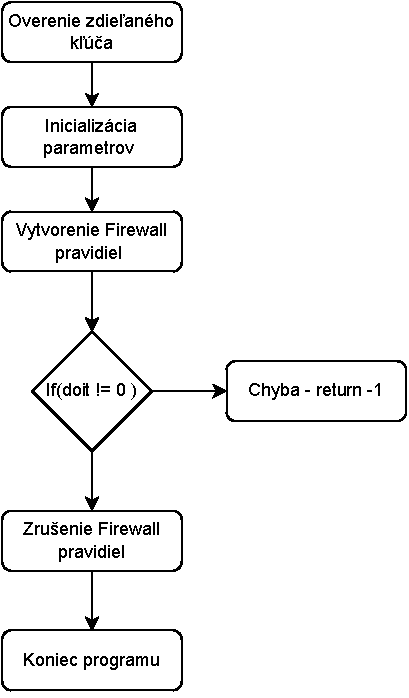
\includegraphics[width=0.5\textwidth]{figures/fc1}
	\caption{Beh DSVPN}
	\label{fc1}
\end{figure}

 Od tohto momentu sa presúvame k postupnému vnáraniu do procesu spojenia a spracovania dát. Vo vnútri \lstinline|doit()| dochádza k vetveniu programu. V prípade, že je DSVPN spustená ako server spustí sa funkcia \lstinline|tcp_listener()|. V opačnom prípade \lstinline|client_reconnect()|. Ulohami funkcií je nastolenie TCP spojenia medzi clientom a serverom. Listener vytvára socket pomocou systemovej funkcie \lstinline|bind()|, ktorý následne čaká na klienta. Smerník na socket je uložený do štruktúry Context. V tejto vetve sa v Context ešte nastaví smerovanie na tento socket. \lstinline|Client_reconnect()| podľa prednastaveného počtu pokusov o znovu nadviazanie spojenia sa pokúša pomocou \lstinline|client_connect()| o spojenie. Pred týmto úkonom samozrejme dochádza k overeniu či už nedošlo k nadviazaniu spojenia a o to sa stará \lstinline|client_disconnect()|.


 
  \lstinline|Client_connect()| slúži na pripojenie klienta k serveru. Vykonáva úpravu pravidiel v \acrshort{fw}. Následne sa pokúša o nadviazania spojenia pomocou funkcie  \lstinline|tcp_client()|. Po tejto sérií úloh sa vraciame opäť do \lstinline|doit()|. Tu je vo  \lstinline|while| cykle vykonávaná funkcia \lstinline|event_loop()|, v ktorej dochádza k použitiu kryptografickej knižnice charm. Jej obsahom je inicializácia premenných. viď. \ref{el}. Schéma \ref{fc2} znázorňuje opísané skutočnosti.
  
  \begin{minipage}{\linewidth} 	
  	\begin{lstlisting}[frame=single,
  		numbers=left,
  		caption={Premenné funkcie event loop}\label{el},
  		basicstyle=\ttfamily\small, keywordstyle=\color{black}\bfseries,]
     struct pollfd *const fds = context->fds;
  Buf                  tun_buf;
  Buf *                client_buf = &context->client_buf;
  ssize_t              len;
  int                  found_fds;
  int                  new_client_fd;
    	\end{lstlisting}
\end{minipage}\\ 
 
 

\begin{figure}
	\centering
	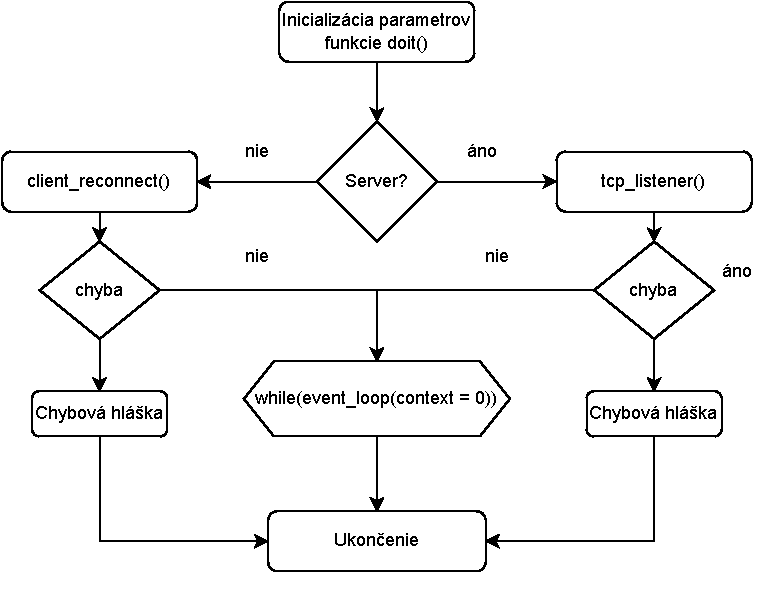
\includegraphics[width=0.9\textwidth]{figures/fc2}
	\caption{Funkcia Doit()}
	\label{fc2}
\end{figure}

 \subsubsection{Funckia event\_loop()}
 Event\_loop je 111 riadkov dlhá funkcia. Jej obsah môžeme rozdeliť na overovací a výkonový. Úlohou niekoľkých if-ou vo funkcii je preverovanie signálov, spätných hodnôt a podobných premenných, ktoré by signalizovali chybu alebo používateľov záujem o ukončenie relácie programu. 
 
 Zaujímavé je taktiež predom definované makro \lstinline|BUFFERBLOAT_CONTROL|. Jeho úlohou je zamedzenie problému zvaného \textbf{Bufferbloat}. V skratke, je to nechcený jav, ktorý je zapríčinený nadmerným ukladaním paketov do vyrovnávacej pamäte, tzv. zahltenie. To ma za následok vysokú latenciu a tzv. Packet Delay Variation -- \acrshort{pdv} (Jitter), v paketovo-orientovaných sieťach. Viac o tejto problematike je možne si prečítať na \cite{bufferbloat}.
 
 Na druhej strane výkonové funkcie, ako hovorí ich názov. niečo vykonávajú. Do tejto kategórie sme zaradili funkcie:
 \begin{itemize}
 	\item\lstinline|tcp_accept()| -- slúži na nastolenie nového TCP spojenia s klientom, 
 	\item\lstinline|tun_read()| -- volá \lstinline|safe_read_partial| v prípade linuxového OS,
 	\item\lstinline|uc_encrypt()| -- kryptografické šifrovanie správy,
 	\item\lstinline|safe_write_partial()| -- používa štandardizovanú funkciu write vo while cykle, zapíše zašifrované dáta do buffera určeného pre odoslanie klientovi, vracia počet zapísaných dát,
 	\item\lstinline|safe_write()| -- používa sa v prípade ak došlo k zahlteniu paketmi,
 	\item\lstinline|client_reconnect()| -- slúži na obnovu spojenia v prípade chyby,
 	\item\lstinline|safe_read_partial()| -- obdobne ako pri write, používa read funkciu,
 	\item\lstinline|uc_decrypt()| -- kryptografické dešifrovanie správy,
 	\item\lstinline|tun_write()| -- volá \lstinline|safe_write| pri OS Linux.
 \end{itemize}
Metóda použitá pri zápise zašifrovaných dát vo funkcii \lstinline|event_loop()| je znázornená v \ref{ed}.

 \begin{minipage}{\linewidth} 	
 	\begin{lstlisting}[frame=single,
 		numbers=left,
 		caption={Spôsob zápisu šifrovaných dát}\label{ed},
 		basicstyle=\ttfamily\small, keywordstyle=\color{black}\bfseries,]
 		
 writenb = safe_write_partial(context->client_fd, tun_buf.len,
 			    	 		         		  2U + TAG_LEN + len); 
 if (writenb < (ssize_t) 0) {// kontrola zahltenia -- bufferbloat
 	context->congestion = 1; 
 	writenb             = (ssize_t) 0;
 }
// ak je iny objem ako maximum
 if (writenb != (ssize_t)(2U + TAG_LEN + len)) {
 	writenb = safe_write(context->client_fd, tun_buf.len + writenb,
 	2U + TAG_LEN + len - writenb, TIMEOUT); 
 }
   	\end{lstlisting}
\end{minipage}\\ 
 
\subsubsection{Šifrovanie a dešifrovanie}
Proces šifrovanie resp. dešifrovania správy nastáva na oboch stránách siete, teda pri klientovy aj serveri. \ref{SS} demonštruje šifrovanie implementované v funkcii \lstinline|uc_encrypt()|. Tento proces sme sa pokúsili opísať v grafe \ref{fc3}. 

\begin{figure}
	\centering
	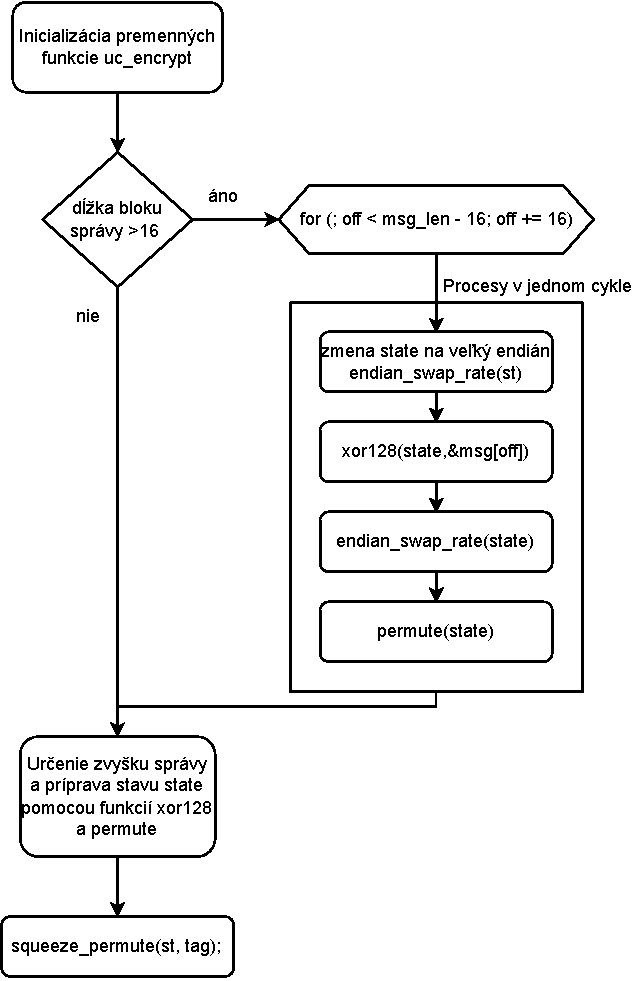
\includegraphics[width=0.7\textwidth]{figures/fc3}
	\caption{Funkcia uc\_encrypt}
	\label{fc3}
\end{figure}

\begin{minipage}{\linewidth} 	
	\begin{lstlisting}[frame=single,
		numbers=left,
		caption={Šifrovanie správy}\label{SS},
		basicstyle=\ttfamily\small, keywordstyle=\color{black}\bfseries,]
 		
void uc_encrypt(uint32_t st[12], unsigned char *msg, 
					      size_t msg_len, unsigned char tag[16])
{	//spracovanie po 16 znakov
	unsigned char squeezed[16];
	unsigned char padded[16 + 1];
	size_t        off = 0;
	size_t        leftover;
	
	if (msg_len > 16) {
		for (; off < msg_len - 16; off += 16) {
			endian_swap_rate(st);
			memcpy(squeezed, st, 16);
			xor128(st, &msg[off]);
			endian_swap_rate(st);
			xor128(&msg[off], squeezed);
			permute(st);
		}
	}
	leftover = msg_len - off;
	memset(padded, 0, 16);
	mem_cpy(padded, &msg[off], leftover);
	padded[leftover] = 0x80;
	endian_swap_rate(st);
	memcpy(squeezed, st, 16);
	xor128(st, padded);
	endian_swap_rate(st);
	st[11] ^= (1UL << 24 | (uint32_t) leftover >> 4 << 25
				    | 1UL << 26); 
	xor128(padded, squeezed);
	mem_cpy(&msg[off], padded, leftover);
	permute(st);
	squeeze_permute(st, tag);
}
  	\end{lstlisting}
\end{minipage}\\ 

Ako je viditeľne v kóde dochádza k častému použitiu 2 funkcií. Nimi sú  \lstinline|xor128()| a  \lstinline|permute()|. Jedná sa o pomerne dôležité bloky pre správne fungovanie šifrovacieho algoritmu. Obsah prvej z uvedených je preto znázornený v \ref{xor}.

\begin{minipage}{\linewidth} 	
	\begin{lstlisting}[frame=single,
		numbers=left,
		caption={Funkcia xor128}\label{xor},
		basicstyle=\ttfamily\small, keywordstyle=\color{black}\bfseries,]
static inline void xor128(void *out, const void *in)
{
	#ifdef __SSSE3__
	_mm_storeu_si128((__m128i *) out,
	_mm_xor_si128(_mm_loadu_si128((const __m128i *) out),
	_mm_loadu_si128((const __m128i *) in)));
	#else
	unsigned char *      out_ = (unsigned char *) out;
	const unsigned char *in_  = (const unsigned char *) in;
	size_t               i;
	
	for (i = 0; i < 16; i++) {	//xororvanie jednotlivych znakov 
		out_[i] ^= in_[i];		//v 16 bitovom bloku spravy
	}
	#endif
}
  	\end{lstlisting}
\end{minipage}\\ 

Na druhej strane \lstinline|permute()| je pomerne rozsiahla funkcia pričom jej obsah sa rozprestiera na 100 riadkoch. Funkcionalita závisí od procesorových inštrukcií. Avšak nás bude zaujímať softvérová implementácia, ktorá je aj použitá pri behu. Dôvodom je, že naše zariadenie nemá k dispozícií uvedené procesorové inštrukcie. Blok, ktorý je použitý pri volaní sa nachádza v \ref{permute}.   

\begin{minipage}{\linewidth} 	
	\begin{lstlisting}[frame=single,
		numbers=left,
		caption={Funkcia Permute + makrá }\label{permute},
		basicstyle=\ttfamily\small, keywordstyle=\color{black}\bfseries,]
#define ROTR32(x, b) (uint32_t)(((x) >> (b)) | ((x) << (32 - (b))))
#define SWAP32(s, u, v)        \
do {                           \
	t      = (s)[u];             \
	(s)[u] = (s)[v], (s)[v] = t; \
} while (0)
	
static void permute(uint32_t st[12])
{
	uint32_t e[4], a, b, c, t, r, i;	
	for (r = 0; r < XOODOO_ROUNDS; r++) {
		for (i = 0; i < 4; i++) {
			e[i] = ROTR32(st[i] ^ st[i + 4] ^ st[i + 8], 18);
			e[i] ^= ROTR32(e[i], 9);
		}
		for (i = 0; i < 12; i++) {
			st[i] ^= e[(i - 1) & 3];
		}
		SWAP32(st, 7, 4);
		SWAP32(st, 7, 5);
		SWAP32(st, 7, 6);
		st[0] ^= RK[r];
		for (i = 0; i < 4; i++) {
			a         = st[i];
			b         = st[i + 4];
			c         = ROTR32(st[i + 8], 21);
			st[i + 8] = ROTR32((b & ~a) ^ c, 24);
			st[i + 4] = ROTR32((a & ~c) ^ b, 31);
			st[i] ^= c & ~b;
		}
		SWAP32(st, 8, 10);
		SWAP32(st, 9, 11);
	}	
}
	\end{lstlisting}
\end{minipage}\\ 
\section{Analýza výpočtových nárokov DSVPN}\label{analyza}
mozno sekcia nie kapitola, K VPN neviem co pozerat 
https://windowsreport.com/test-vpn/ \\
https://www.mdpi.com/1999-5903/14/9/264 \\
https://nordvpn.com/vpn-speed-test/ \\
https://ieeexplore.ieee.org/stamp/stamp.jsp?tp=\&arnumber=9142755 \\
https://citeseerx.ist.psu.edu/document?repid=rep1\&type=pdf\&doi=a5639b03df528315a8e901f8f6b2bad2824a643a \\

\section{Windows kompatibilita}
za ucelom Creating a virtual network device similar to /dev/net/tun in C on Windows

To use the OpenVPN/tap-windows driver in a C program, you need to first install the driver on your Windows system. You can download the driver from the OpenVPN website.

Once the driver is installed, you can use the following code snippet to create and configure a tap interface in your C program:

This code snippet opens the tap adapter with the name "tap0801", queries and sets the media connect status, and then closes the adapter. You can modify the code to suit your specific needs.

adapter

 https://github.com/OpenVPN/tap-windows/tree/master/installer
 \subsection{2.option}
 On Linux, /dev/net/tun is used to create virtual network devices. On Windows, the equivalent is the TAP-Windows driver used by OpenVPN. To create a virtual network device on Windows using TAP-Windows driver, you can use the following code as an example:
 

 Note that this code uses the TAP-Windows driver's control device interface to configure and set the status of the virtual network device. It opens the TAP device using the path "\\\\.\\Global\\TAP-Windows6" and sends the appropriate control codes to the device using the DeviceIoControl function. The TAP\_IOCTL\_CONFIG\_TUN control code is used to configure the TAP device, and the TAP\_IOCTL\_SET\_MEDIA\_STATUS control code is used to set the device status to up. The virtual network device name is returned by the TAP device driver and can be obtained from the tapName variable after calling TAP\_IOCTL\_CONFIG\_TUN.
\section{incode creation }